%-------------------------------------------------------------------------------
%-------------------------------------------------------------------------------
\begin{frame}\begin{center}
	\LARGE\textbf{Housekeeping}
\end{center}\end{frame}
%-------------------------------------------------------------------------------
%-------------------------------------------------------------------------------
\begin{frame}
	\textbf{Course Website}\vspace{0.3cm}

You find all information about the course on our website.

\begin{center}
\url{https://github.com/HumanCapitalEconomics}
\end{center}

This includes the lecture dates, topics, reading list, and the slides.\vspace{0.3cm}

If you have further questions, please feel free to contact us using

\includegraphics[scale=0.5]{../../shared/fig-gitter}.

\end{frame}
%-------------------------------------------------------------------------------
%-------------------------------------------------------------------------------
\begin{frame}

\begin{itemize}\setlength\itemsep{1em}
\item What happened in the last lecture?
\item How does it relate to what we are doing this week?
\end{itemize}

\end{frame}
%-------------------------------------------------------------------------------
%-------------------------------------------------------------------------------
\begin{frame}
\begin{figure}[htp]\centering
	\caption{Modeling process}\scalebox{0.45}
	{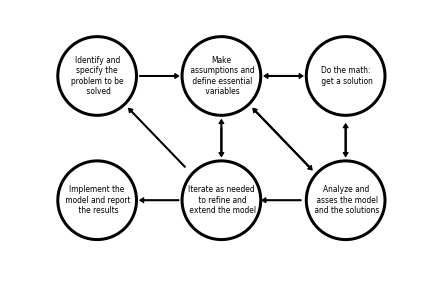
\includegraphics{../../01_introduction/material/fig-modeling-process}}
\end{figure}

\end{frame}
%-------------------------------------------------------------------------------
%-------------------------------------------------------------------------------
\begin{frame}
\textbf{Multidimensionality of skills}\vspace{0.3cm}

\begin{itemize}
\item \bibentry{Heckman.2006b}
\item \bibentry{Eisenhauer.2015b}
\end{itemize}


\end{frame}
%-------------------------------------------------------------------------------
%-------------------------------------------------------------------------------
\begin{frame}

\begin{center}
{\fontsize{125}{60}\selectfont ?}
\end{center}

\end{frame}
%-------------------------------------------------------------------------------
%-------------------------------------------------------------------------------
